\documentclass[pscyr,nonums]{hedlab}
\usepackage[russian]{babel}
\usepackage[utf8]{inputenc}
\usepackage{graphicx}
\usepackage{listings}
\usepackage{hedmaths}

\labnum{3}
\labname{Метод имитации отжига}
\student{Чечеткин И. А.}
\labdate{}

\begin{document}
  \makeheader
  \lstset{language=python, basicstyle=\tiny, numbers=left }

  \noindent\emph{Цель работы:} 
  \begin{enumerate}
    \item познакомиться с методом имитации отжига;
    \item реализовать алгоритм на языке программирования;
    \item получить значения минимума функции на некоторых входных данных.
  \end{enumerate}

  Исследуемая функция:
  \[
    f(x, y) = x^2 + 5\frac{\abs{x}}{\sqrt{\abs{x} + 0.1}} +
      \frac{\abs{x - 0.2}}{\sqrt{\abs{x - 0.2} + 0.01}} +
      \frac{\abs{x + 0.2}}{\sqrt{\abs{x + 0.2} + 0.01}} + y^2.
  \]

  График исследуемой функции:
  \begin{figure}[h!]
    \centering
    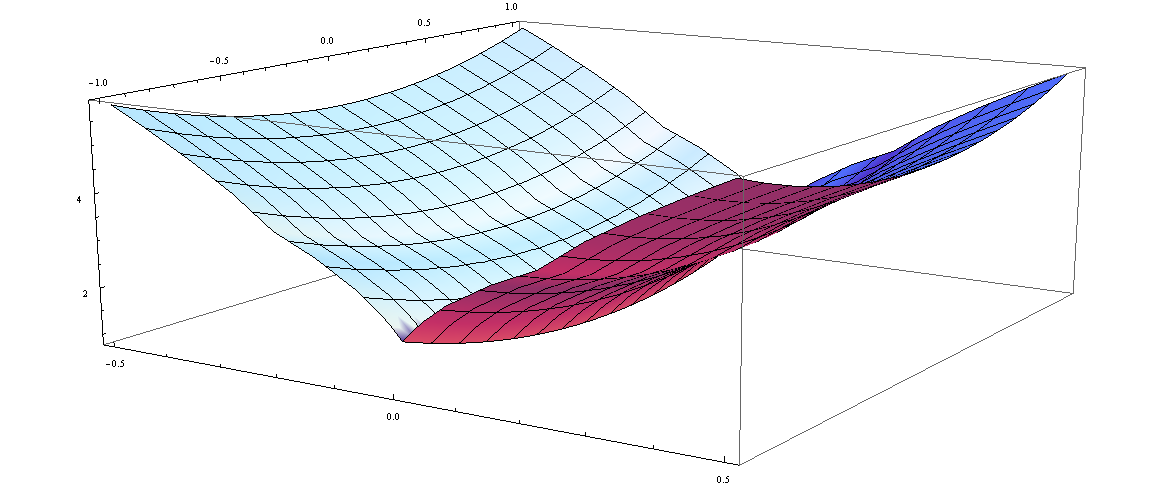
\includegraphics[width=.8\textwidth]{graph}
  \end{figure}

  Полученные результаты:
  \begin{table}[h!]
    \center
    \begin{tabular}{|*{6}{c|}} \hline
      радиус поиска R & температура T & кол-во итераций N & 
        x & y & f(x, y) \\ \hline
      2.0 & 1.0   & 100 & -0.164146 &  0.299630 &  2.476386 \\ \hline
      1.0 & 20.0  & 50  &  0.276907 & -1.074900 &  4.431628 \\ \hline
      1.0 & 100.0 & 50  & -0.213127 & -2.945829 & 11.349116 \\ \hline
      0.5 & 100.0 & 25  &  0.000254 &  0.826744 &  1.560382 \\ \hline
      1.0 & 1.0   & 100 &  0.006295 &  0.034139 &  0.970501 \\ \hline
      0.5 & 100.0 & 10  &  0.160743 &  0.201890 &  2.409911 \\ \hline
      0.3 & 1.0   & 100 & -0.011509 & -0.465819 &  1.261922 \\ \hline
    \end{tabular}
  \end{table}
  
  Рассчитанный с помощью мат. пакета минимум: 0.872872 при
  \( x = 0,\ y = 0 \).

  \clearpage

  \noindent Исходный код программы
  \lstinputlisting{annealing.py}
\end{document}
